\section*{(Sequential) importance sampling}
The central idea of Particle filters is to represent the posterior of
the system $p(x_k \mid y_{1:k})$ at some time $k$ as a weighted set of
samples, so called \emph{particles}, denoted by
$\{ x^{(i)}_k; w^{(i)}_k \}$. If we ignore for a moment the weights
and assume that the samples are from the desired distribution, \ie,
\[
  x^{(i)}_k \sim p(x_k^{(i)} \mid y_{1:k}), \quad i = 1, \dotsc, N
\]
the Monte Carlo method approximates $p(x_k \mid y_{1:k})$ by the
empirical measure\footnote{Again, we slightly abuse notation for the
  sake of simplicity and refrain from a rigorous measure-theoretic
  formulation.}
\begin{equation}
  \label{eq:empirical_measure}
  \hat{p}(x_k \mid y_{1:k}) = \frac{1}{N} \sum_{i = 1}^N
  \delta_{x_k^{(i)}}(x_k)\,,
\end{equation}
where $\delta_x(\cdot)$ denotes the Dirac delta centred at $x$. The
expectation of a test function $f : \R^{d_x} \rightarrow \R$ given by
\[
  \mathbb{E}[f(x_k) \mid y_{1:k}] = \int f(x_k) p(x_k \mid y_{1_k})
  \dx_k
\]
is then estimated by
\[
  {\mathbb{E}}^{\text{MC}}[f(x_k) \mid y_{1:k}] = \int f(x_k)
  \hat{p}(x_k \mid y_{1_k}) \dx_k = \frac{1}{N} \sum_{i=1}^N
  f(x^{(i)}_k)\,.
\]
It is well-known that the variance of the approximation error using
this estimator decreases \emph{independent of $d_x$} with a rate of
$\mathcal{O}(N^{-1})$. However, often it is either impossible or
practically intractable to sample from the posterior directly and
thus, one often relies on a technique called \emph{importance
  sampling}.

We start by choosing an \emph{importance density}
$q(x_k \mid y_{1:k})$ and draw $N$ samples $x^{(i)}_k$,
$i = 1, \dotsc, N$ from it. If we would use these samples to
approximate $p(x_k \mid y_{1:k})$ as in~\eqref{eq:empirical_measure}
the result would obviously not be accurate in general. To correct this
bias we introduce \emph{importance weights}
\begin{equation}
  \label{eq:importance_weights}
  w_k^{(i)} \propto \frac{p(x_k^{(i)} \mid y_{1:k})}{q(x_k^{(i)} \mid
    y_{1:k})} \,,
\end{equation}
that we require to be normalised such that $\sum_i w_k^{(i)} = 1$. We
can now approximate the target density by
\begin{equation}
  \label{eq:karget:approx}
  p(x_k \mid y_{1:k}) \approx \sum_{i=1}^N w_k^{(i)} \delta_{x_k^{(i)}}(x_k) \,.
\end{equation}
This technique is called \emph{importance sampling}. Expectations of
test functions can then be estimated by
\[
  \mathbb{E}^{\text{MC}}[f(x_k) \mid y_{1:k}] = \sum_{i=1}^N
  w_k^{(i)}f(x_k^{(i)}) \,.
\]
Due to assumption (A3) ideally we would like a recursive formula to
update the weights at each step. To obtain such a formula we consider
the full posterior $p(x_{0:k} \mid y_{1_k})$ and express it in terms
of the posterior at the previous time step and the known pdfs
$p(y_k \mid x_k)$ and $p(x_k \mid x_{k-1})$:
\begin{align*}
  p(x_{0:k} \mid y_{1:k}) &\propto p(y_k \mid x_{0:k}, y_{1:k-1}) p(x_{0:k} \mid y_{1:k-1}) \\
                          &= p(y_k \mid x_k) p(x_k \mid x_{0:k-1}, y_{1:k-1}) p(x_{0:k-1} \mid y_{1:k-1}) \\
                          &= p(y_k \mid x_k) p(x_k \mid x_{k-1}) p(x_{0:k-1} \mid y_{1:k-1})\,,
\end{align*}
where we used Bayes' theorem and the properties of the system
described earlier (see~\cite{arulampalam} for a more detailed
derivation). If in addition we choose an importance density that
factorises such that
\[
  q(x_{0:k} \mid y_{1:k}) = q(x_k \mid x_{0:k-1}, y_{1:k}) q(x_{0:k-1}
  \mid y_{1:k-1})
\]
the weights~\eqref{eq:importance_weights} can be written as
\begin{align*}
  w_k^{(i)} &\propto \frac{p(y_k \mid x_k^{(i)}) p(x_k^{(i)} \mid x_{k-1}^{(i)}) p(x_{0:k-1}^{(i)} \mid y_{1:k-1})}{q(x_k^{(i)} \mid x_{0:k-1}^{(i)}, y_{1:k}) q(x_{0:k-1}^{(i)} \mid y_{1:k-1})} \\
            &= \frac{p(y_k \mid x_k^{(i)}) p(x_k^{(i)} \mid x_{k-1}^{(i)})}{q(x_k^{(i)} \mid x_{0:k-1}^{(i)}, y_{1:k})} w^{(i)}_{k-1} \,.
\end{align*}
Since we are only interested in estimating the filtered posterior
$p(x_k \mid y_{1:k})$ we choose an importance density
$q(x_k \mid x_{0:k-1}, y_{1:k}) = q(x_k \mid x_{k-1}, y_{k})$ that
only depends on $x_{k-1}$ and $y_k$. Then, it suffices to only keep
$x_k^{(i)}$ in memory while the path $x_{0:k-1}^{(i)}$ and history of
observations $y_{1:k-1}$ can be discarded. The weights can recursively
be computed by
\begin{equation}
  \label{eq:weight_update}
  w_k^{(i)} \propto \frac{p(y_k \mid x_k^{(i)}) p(x_k^{(i)} \mid
    x_{k-1}^{(i)})}{q(x_k^{(i)} \mid x_{k-1}^{(i)}, y_{1:k})}
  w^{(i)}_{k-1} \,.
\end{equation}
This is usually referred to as \emph{sequential} importance sampling.
We summarise the results up to this point in Algorithm~\ref{alg:sis}.
Note that since at time $k = 0$ no observation or previous state is
available, we sample from the (known) prior and weigh all particles
equally.
\begin{algorithm}[t]
  \SetAlgoLined \KwData{$n$ observations $y_1, y_2, \dotsc, y_n$;\quad
    number of particles $N$}
  Sample $x_0^{(i)} \sim p(x_0^{(i)})$ \;
  Set weights $w_0^{(i)} = 1/N$\;
  \For{$k = 1,2, \dotsc, n$}{
    Sample $x_k^{(i)} \sim q(x_k^{(i)} \mid x_{k-1}^{(i)}, y_k)$. \;
    Compute unnormalised weights $\tilde{w}_k^{(i)}$ according to~\eqref{eq:weight_update} \;
    Normalise $w_k^{(i)} = \tilde{w}_k^{(i)} / \sum_j \tilde{w}_k^{(j}$\;
  }
  \caption{Sequential importance sampling}\label{alg:sis}
\end{algorithm}

Using this approach alone, however, leads to \emph{degeneracy} of the
particles. It can be shown that the variance of the weights can only
increase at every step~\cite[Proposition 1]{Doucet2000} which implies
that the algorithm will eventually produce a single non-zero weight
$w^{(i)} = 1$, carrying all the statistical information. This is
visualised in Figure~\ref{fig:weights} where we plotted a histogram of
the weights after the first few time steps using the model described
later in Example~\ref{ex:lv1}. One can clearly see that after a few
steps almost all of the weights are zero. To account for this problem,
we introduce another technique called \emph{resampling}.
\begin{figure}
  \centering
  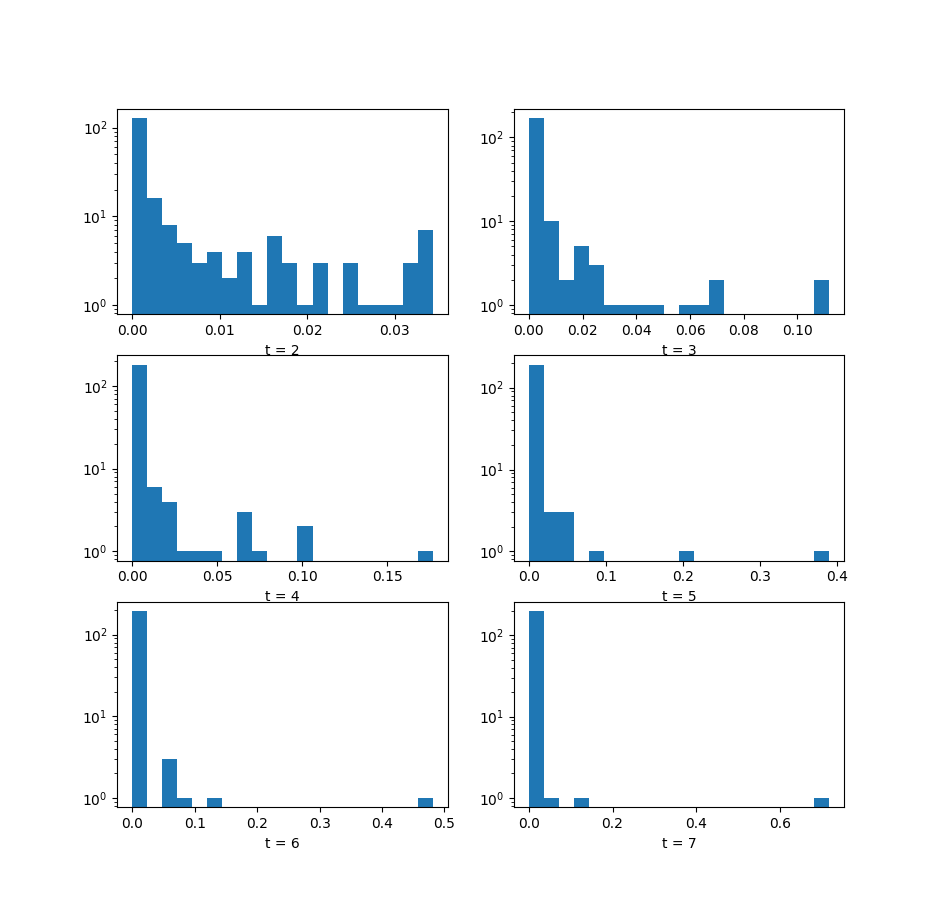
\includegraphics[width=\textwidth]{figures/Figure_weights.png}
  \caption{A histogram of 200 weights after just a few
    iterations. Almost all of the weights are zero at $k = 7$ which
    demonstrates the degeneracy of the particles.}%
  \label{fig:weights}
\end{figure}

%%% Local Variables:
%%% mode: latex
%%% TeX-master: "../main"
%%% End:
